\documentclass[12pt]{article} % 12pt is standard for thesis readability

% --- Layout & Margins ---
\usepackage[a4paper, margin=1in]{geometry} % Standard 1-inch margins for thesis

% --- Packages for Tables and Figures ---
\usepackage{graphicx} % Required for \resizebox
\usepackage{booktabs} % Required for professional table lines (\toprule, etc.)
\usepackage{multirow}
\usepackage{listings}
\usepackage{placeins}
\lstset{
  inputencoding=utf8,
  extendedchars=true,
  literate=
    {ä}{{\"a}}1
    {ö}{{\"o}}1
    {ü}{{\"u}}1
    {Ä}{{\"A}}1
    {Ö}{{\"O}}1
    {Ü}{{\"U}}1
    {ß}{{\ss}}1
}
\usepackage[
    backend=biber,
    style=authoryear,      % Fixed: Changed from 'unified' to standard 'authoryear' to prevent engine crash
    maxcitenames=3,    
    maxbibnames=99,
    uniquename=init,            
    uniqueprimaryauthor=true]{biblatex}
\addbibresource{literature.bib}
\DeclareNameFormat{labelname}{%
  % Schalte die Unterscheidung (uniquename) temporär ab (auf 0), wenn:
  % 1. der Autor ein Co-Autor ist (listcount > 1) ODER
  % 2. der Nachname des Erstautors unter allen Erstautoren eindeutig ist.
  \ifboolexpr{test {\ifnumcomp{\value{listcount}}{>}{1}} or test {\ifuniqueprimaryauthor}}
    {\setcounter{uniquename}{0}}
    {}%
  \ifcase\value{uniquename}%
    \usebibmacro{name:family}
      {\namepartfamily}
      {\namepartgiven}
      {\namepartprefix}
      {\namepartsuffix}%
  \or
    \ifuseprefix
      {\usebibmacro{name:given-family}
        {\namepartfamily}
        {\namepartgiveni}
        {\namepartprefix}
        {\namepartsuffix}}
      {\usebibmacro{name:given-family}
        {\namepartfamily}
        {\namepartgiveni}
        {\namepartprefixi}
        {\namepartsuffix}}%
  \else
    \usebibmacro{name:given-family}
      {\namepartfamily}
      {\namepartgiven}
      {\namepartprefix}
      {\namepartsuffix}%
  \fi
  \usebibmacro{name:andothers}}

\usepackage{amsmath}

\title{Optimizing RAG Pipelines for Small Language Models\\[0.3cm]
       \large Evaluating Document Preprocessing, Chunking, and Query Expansion on Structured Administrative Data}

\author{Daniel Gelderblom}
\date{May 2026}

\begin{document}

\begin{titlepage}
    \begin{center}
        % --- Header Information ---
        {\large Bachelorarbeit im Studiengang Computerlinguistik (B.A.)\\[0.2cm]
            an der Heinrich-Heine-Universität Düsseldorf}

        \vfill

        % --- Logo ---
        
\includegraphics[width=0.35\textwidth]{images/logo-hhu.png}

        \vfill

        % --- Title & Subtitle ---
        {\Huge \bfseries Optimizing RAG Pipelines for Small Language Models}\\[0.4cm]
        {\large Evaluating Document Preprocessing, Chunking, and Query Expansion\\[0.15cm]
        on Structured Administrative Data}

        \vfill
        \vfill

        % --- Author & Submission Details ---
        \begin{tabular}{c}
            \textbf{vorgelegt von:}        \\[0.2cm]
            Daniel Gelderblom              \\
            Otto-Hahn-Straße 118           \\
            40591 Düsseldorf               \\
            \url{Daniel.Gelderblom@hhu.de} \\
            Matrikelnummer: 3131057
        \end{tabular}

        \vfill

        % --- Advisors & Date ---
        \begin{tabular}{rl}
            \textbf{Abgabedatum:}     & 21. September 2026        \\[0.15cm]
            \textbf{Erstgutachterin:} & Prof. Dr. Wiebke Petersen \\
            \textbf{Zweitgutachter:}  & David Arps
        \end{tabular}
    \end{center}
\end{titlepage}

\newpage

% set page number to 1
\setcounter{page}{1}
% Hier römisch zählen, unten ab 1
\pagenumbering{roman}
\pagestyle{plain}
\tableofcontents
\listoffigures

\listoftables
\newpage
\pagenumbering{arabic}

\section{Introduction}
Since the publication of OpenAI's GPT-3 \parencite{gpt3_openai}, Large Language Models (LLMs) have gained immense importance. A major problem with LLMs, however, is their tendency to hallucinate. Especially in contexts like user queries on specific documents, factual correctness is vital.\\
Before the rise of transformer-based LLMs, language models had received all the knowledge during training. \textcite{guu2020retrieval} first used retrieval from a knowledge base together with generation during training, thus not needing to train the model on all knowledge. \textcite{karpukhin2020dense}
improved dense retrieval (retrieval based on similarity scores of text embeddings), making it better than keyword-based retrieval and thus completing the foundation for Retrieval Augmented Generation (RAG). RAG \parencite{lewis2020retrieval} combines a (most often dense) retriever with a generational model. The retriever takes documents from a knowledge base relevant to a query and feeds them to the text generator to answer the query.\\
As context windows have increased to one million tokens, the need for RAG systems for cutting edge proprietary LLMs, while still present, has decreased. However, these LLMs cannot serve every use-case. When data is confidential, privacy is crucial, and only a locally running language model can be considered. In these settings, resource constraints often apply. Thus, only Small Language Models (SLMs) are an option here. SLMs have smaller context windows (262,144 tokens for the very current Qwen3.5-2B). Far more importantly, due to their small size, they suffer much more from lost-in-the-middle problems. Lost-in-the middle describes the phenomenon where transformer-based language models fail drastically when the answer to a question is placed in the middle of a long prompt \parencite{liu2024lost}. Thus, performance often drops far before reaching the context limit.
For SLMs around 8B parameters, this happens as early as 4000 to 8000 input tokens \parencite{leng2024long}. This means that only a few short documents can be part of the prompt, increasing the importance of a well-designed RAG pipeline, and especially of the retrieval step. Improving this step, specifically through document preprocessing, chunking, and query expansion, is what this work focuses on.\\
Preprocessing is the conversion of documents into a form that is easy for the LLM to understand. Chunking is the technique employed to split the documents, which are all larger than 8000 tokens, into smaller pieces. Query expansion means transforming the query into a form that is easier for the retriever to handle. Thus, the first two parts of the pipeline are only done once for all documents in the offline phase, while query expansion is done for every user input in the online phase (Figure 1).\\
The task at hand is to create a chat-bot to answer administrative questions from students for the Department of Computational Linguistics. The long-term goal is to have this chat-bot run locally on a small GPU. Therefore, only SLMs can be used as generators. Thus, a RAG system with administrative documents as knowledge base is needed. As these documents are in part structured in tables, document preprocessing is a crucial step.\\
Thus, there are several goals for this thesis. Firstly, a RAG pipeline is built. This pipeline should be modular, so new components can be easily added and existing components can be easily improved and changed. Secondly, the best set-up for preprocessing the structured documents is determined empirically. Thirdly, the benefits of query expansion are investigated. Fourthly, possible hyperparameters are evaluated for the chunking algorithms and the best chunking method is determined for the context at hand.
\begin{figure}[htbp]
    \centering
    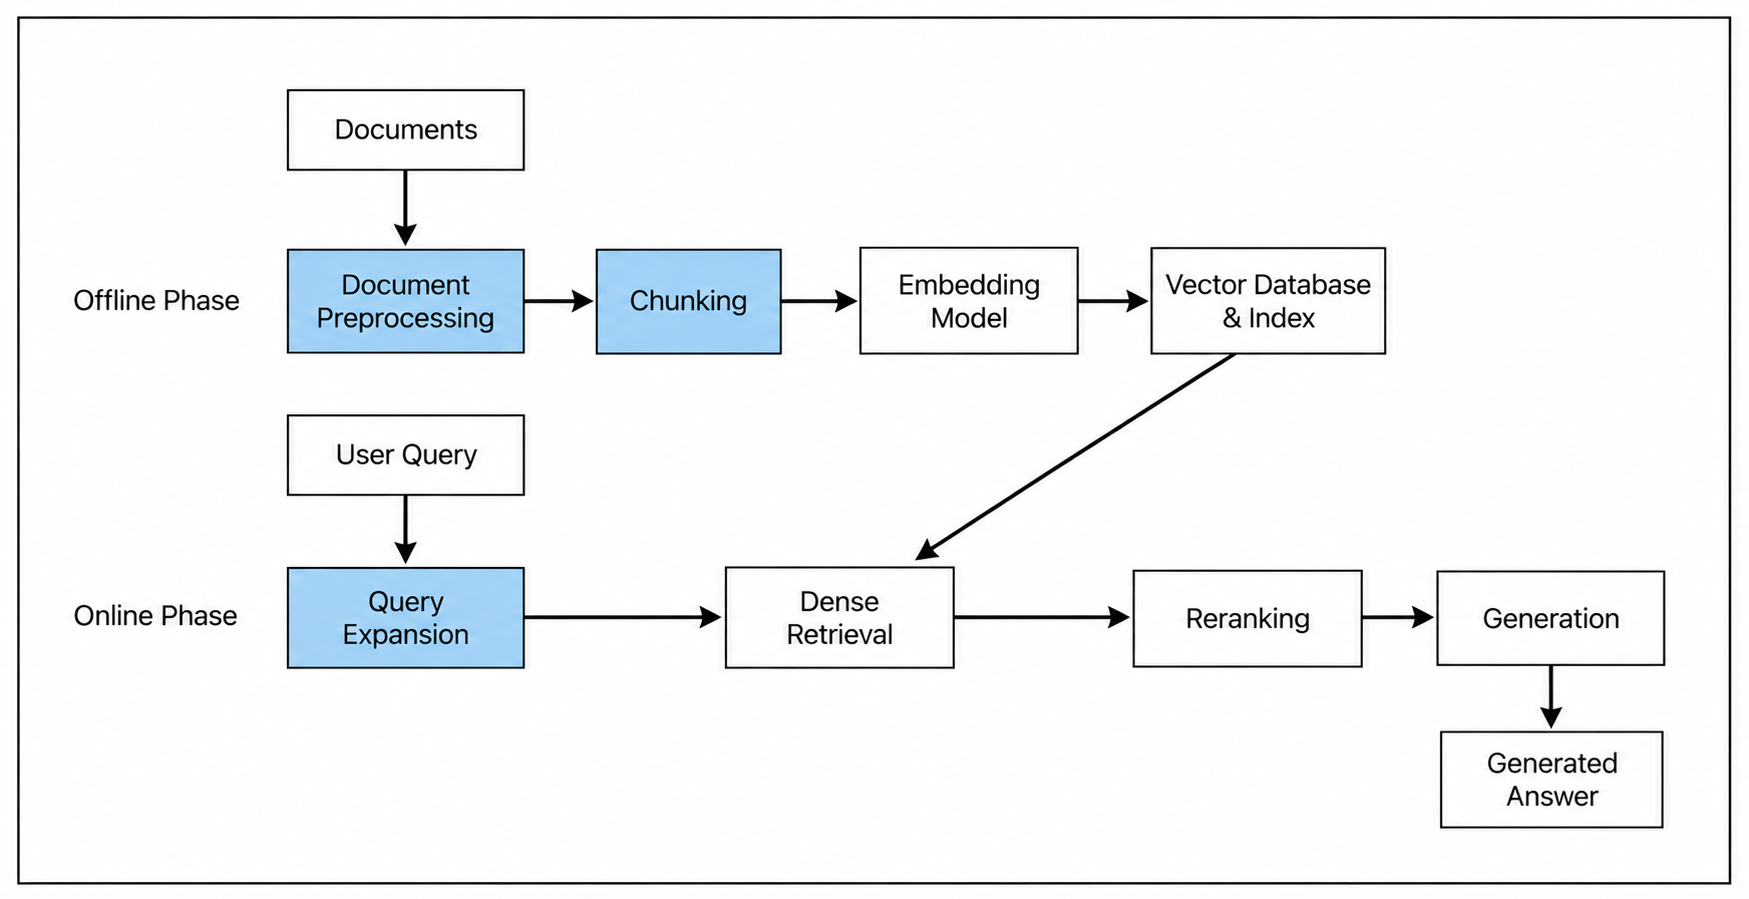
\includegraphics[width=\linewidth]{images/ragpipeline.png}
    \caption{The RAG pipeline}
\end{figure}
\section{Data}
\subsection{Documents}
The RAG-chatbot is based on three administrative documents from the Department of Computational Linguistics at the University of Düsseldorf: Prüfungsordnung (PO), Modulhandbuch (MH) and fachspezifische Prüfungsordnung (fPO)\footnote{The abbreviations are chosen differently in the code due to legacy reasons (Prüfungsordnung was only added later on). In the code, Prüfungsordnung is POges and fachspezifische Prüfungsordnung is PO.}. PO is relatively easy to handle, as it contains all the general information about studying and exams and is structured in paragraphs. MH has to be preprocessed, as all the modules for Computational Linguistics are shown in table-like structures with two columns. For fPO, preprocessing is absolutely crucial as there is a table for every semester containing subjects and their credit points, time required, exams and administrative numbers.


\subsection{Evaluation Dataset}
To benchmark the performance of the RAG pipeline, a domain-specific evaluation dataset comprising 73 question-answer pairs with human-validated gold answers was constructed. The dataset was created in close collaboration with a student representative from the Department of Computational Linguistics. Candidate questions were generated through a combination of self-written queries and hand-selected suggestions produced by Google Gemini, which were subsequently refined to mirror real-world student inquiries. Table~\ref{tab:dataset_samples} provides representative sample pairs illustrating the different topic areas and difficulty profiles present in the evaluation dataset.

The composition of the dataset reflects strategic advice from the student representative, prioritizing topics that represent frequent points of friction throughout the academic life cycle. Consequently, a strong emphasis was placed on questions typical of the early stages of study (Sample pairs 1, 3, 5) and questions about when to take specific courses (Sample pair 1), exams in specific modules (Sample pair 3), and the mandatory internship (Sample pair 4). These topics were combined with broader administrative queries regarding studying in general (Sample pairs 2, 5) and specific questions concerning individual module contents.

To ensure a comprehensive benchmark, the dataset intentionally balances questions across varying levels of retrieval and synthesis difficulty. At the foundational level, it includes easier, direct queries where the answer can be read in one specific location (Sample pairs 2, 4, 5). The dataset also features moderately difficult questions where the target information is located in a single spot but remains hard to find and extract due to dense phrasing or complex tabular structures, particularly information from fPO (Sample pair 3). Finally, the benchmark includes complex queries that require the pipeline to retrieve multiple passages from different sections of a document, interpret them correctly, and synthesize them into a coherent answer, such as assembling a complete first-semester schedule (Sample pair 1).


\begin{table}[htbp]
    \centering
    \small
    \caption{Representative Sample Question-Answer Pairs from the Evaluation Dataset}
    \label{tab:dataset_samples}
    \renewcommand{\arraystretch}{1.3}
    \begin{tabular}{p{0.05\textwidth} p{0.42\textwidth} p{0.45\textwidth}}
        \toprule
        \textbf{\#} & \textbf{User Question}                                                     & \textbf{Gold Answer}                                                                                                                                                                                                                                                             \\
        \midrule
        1           & Welche Kurse sollte ich im ersten Semester belegen?                        & Laut dem exemplarischen Studienverlaufsplan solltest du im ersten Semester folgende Kurse belegen: Mathematische Grundlagen, Einführung in die computationelle Logik, Einführung in die Computerlinguistik, Einführung in die Programmierung mit Python, Morphologie und Syntax. \\
        \midrule
        2           & Bis wann kann ich mich von einer Klausur ohne Angabe von Gründen abmelden? & Von einer Modulprüfung in Form einer Klausur oder einer mündlichen Prüfung kann sich die Kandidatin oder der Kandidat bis spätestens eine Woche vor dem jeweiligen Prüfungstermin abmelden.                                                                                      \\
        \midrule
        3           & Gibt es eine Klausur in Wahrscheinlichkeitstheorie?                        & Nein, im ``Basismodul -- Statistische Methoden in der Computerlinguistik'', zu dem die Wahrscheinlichkeitstheorie gehört, gibt es gar keine Modulprüfung und somit auch keine Klausur. Es müssen lediglich Studienleistungen erbracht werden.                                    \\
        \midrule
        4           & Wann soll ich das Praktikum machen?                                        & Es wird empfohlen, das Berufsfeldpraktikum nach dem vierten oder fünften Semester zu absolvieren.                                                                                                                                                                                \\
        \midrule
        5           & Gibt es eine generelle Anwesenheitspflicht für Vorlesungen?                & Nein, bei Vorlesungen kann keine Anwesenheitspflicht festgelegt werden.                                                                                                                                                                                                          \\
        \bottomrule
    \end{tabular}
\end{table}



\section{RAG pipeline}
\subsection{Code Architecture}
To facilitate systematic experimentation and ensure future extensibility, the codebase of the RAG pipeline is built upon a strictly modular architecture. A fundamental architectural choice is the strict separation of the pipeline into offline and online execution phases. The offline phase handles the computationally expensive, one-time tasks of document preprocessing, chunking, and vector indexing. The online phase manages real-time interactions, encompassing query expansion, retrieval, reranking, and generation.

Each distinct step of the pipeline is encapsulated within its own module using an object-oriented design approach. The architecture relies on abstract base classes for every pipeline component (e.g., preprocessors, chunkers, retrievers, and generators). Specific algorithms and models are implemented as subclasses that inherit from these base classes. This design pattern ensures that replacing an existing component or integrating a new one—such as introducing a hybrid retriever or a novel chunking algorithm—only requires writing a new implementation of the respective base class, leaving the overarching pipeline logic completely untouched.

To manage the high number of possible pipeline configurations, component selection and hyperparameter choices are handled entirely via a central configuration file. A dedicated Python factory script reads this configuration file and dynamically builds the requested pipeline at runtime by instantiating the specified classes. This allows for rapid component switching and modifications of hyperparameters without the need to modify any source code.

Finally, the architecture is designed for easy maintenance of the knowledge base. New PDF files can be seamlessly integrated into the RAG system by simply placing the raw files into a designated documents directory and registering the new document in the configuration file. The factory and offline modules will then automatically process, chunk, and index the new data during the next offline run.
\subsection{Document preprocessing}
As two of the documents contain tables, a direct conversion to raw, unformatted text is not sensible. \textcite{min2024exploring} identified four methods to handle tables for RAG. First, the table can be converted to Markdown. Second, it can be converted to simple sentences using automatic templates.
Third, traditional (non-generative) language models can be finetuned for this task. Fourth, LLMs can be used to convert the tables to linearized text. In a comparison of the four strategies, LLM-based conversion performed best, followed by Markdown, which still gave good generation results.
Thus, for the RAG pipeline, both Markdown and LLM-based conversion are used. For conversion to Markdown, Docling \parencite{Docling} and conversion by an LLM are tested. Docling is a framework based on pre-trained lightweight vision models and a deep learning model specialized on table conversion. The prompt for the conversion via LLM can be found in Listing \ref{lst:markdown_prompt}. \\
\begin{lstlisting}[breaklines=true, basicstyle=\ttfamily,caption={Prompt for conversion to Markdown}, label=lst:markdown_prompt]
Convert this document to markdown. Pay attention to table structure and the separation of tables and modules.
\end{lstlisting}
For conversion to text by an LLM, the technique from Min et al. and a self-written prompt are compared. In the paper, the table is first converted into a nested bracket structure and then converted to text by the LLM. The conversion prompt from the paper is translated into German. The self-written prompt (see Listing~\ref{lst:direct_llm}) takes the documents in Markdown and converts them directly to text.\footnote{Parts of this section have been taken from the previous literature review}
\begin{lstlisting}[breaklines=true, basicstyle=\ttfamily,caption={Prompt for Linearization from Markdown to Text}, label=lst:direct_llm]
Wandle das folgende Markdown-Dokument in klaren, informationsdichten Fließtext um, der für eine semantische Suchmaschine (RAG-Pipeline) optimiert ist.

Befolge dabei strikt diese Regeln:
1. Informationserhalt: Übernimm ausnahmslos jede Information, jede Zahl und jedes Detail.
2. Hohe Entitätsdichte (WICHTIG): Vermeide Pronomen (er, sie, es, diese) über Absatzgrenzen hinweg. Wiederhole stattdessen immer wieder die konkreten Eigennamen, Produktnamen oder Fachbegriffe, damit jeder Absatz auch isoliert verständlich bleibt.
3. Tabellen & Listen: Wandle Tabellen und Aufzählungen in zusammenhängende Textabsätze um. Formuliere die Beziehungen zwischen Spalten/Zeilen in ganzen Sätzen aus.
4. Überschriften als Kontext: Nutze Überschriften, um den darauffolgenden Absatz mit einem klaren Kontext-Satz zu beginnen (z. B. statt nur "Spezifikationen:" -> "Die technischen Spezifikationen des Geräts X umfassen...").
5. Formatierung: Entferne alle Markdown-Zeichen (*, #, -, |). Behalte klare Absatzumbrüche bei, um logische Trennungen beizubehalten.

Input Text:
---
{text}
---
\end{lstlisting}
\subsection{Chunking}
With early transformer models and the first RAG systems, chunking was only done in a fixed size of tokens, words or characters \parencite{dai2019transformer, lewis2020retrieval}. For this thesis, Fixed Character Chunking was implemented as a baseline chunker. With Dynamic Token Chunking and Fixed Paragraph Chunking, two other simple deterministic Chunkers were implemented. Dynamic Token Chunking sets a maximum number of tokens and cuts off at the last sentence ending before the limit. Fixed Character Chunking packs a fixed number of paragraphs into one chunk. Fixed Character Chunking and Fixed Paragraph Chunking are used in combination with both preprocessing techniques, while Dynamic Token Chunking is only used with linearized text, as it needs sentences for splitting and does not work with Markdown tables.\\
A big problem of chunking in general, and especially fixed-size chunking, is the splitting of contexts (context problem). A word or a sentence in one chunk can reference parts of the previous chunk or even a more distant one. This information gets lost in the chunking process. The first solution to this problem, which was derived from the training of BERT \parencite{devlin2019bert}, was overlapping chunks. Overlap is a certain number of tokens or characters that two adjacent chunks share, giving the beginning and the end of a chunk more context. For Fixed Character Chunking, Fixed Paragraph Chunking, and Dynamic Token Chunking, an overlap is tested in the experiments.\\
Another solution to the context problem is semantic chunking. This method embeds every sentence and separates two adjacent sentences into different chunks if their similarity is below a certain threshold \parencite{kamradt2024fivelevels}. However, later studies found that semantic chunking had only a slight, non-significant edge over fixed-size chunking for large contexts, which does not justify the computational overhead \parencite{qu2025semantic,bennani2026systematic}. This led to the development of Max-Min-Chunking, an improved semantic chunker achieving significantly better retrieval and RAG accuracy than both previous semantic chunkers and simple fixed-size chunkers. The algorithm uses "dynamic clustering". With Max-Min semantic chunking, a sentence is allocated to the same chunk as the previous one if it shares a higher similarity with any sentence in the current chunk than the pair with the lowest similarity in the chunk. This dynamic threshold can even be dampened or increased by a factor c. It is also getting higher with increasing chunk size through a sigmoid-based function. There is, however, a hard baseline for cosine similarity (fixed\_threshold). The Max-Min chunker is tested for linearized text in the chunking experiments.\\
An alternative approach to deal with the context problem is improving the workflow of chunking. Contextual Retrieval addresses it by prepending contextual text to every chunk, situating it inside the bigger document. This significantly reduces the retrieval failure rate \parencite{anthropic2024contextual}. JinaAI proposed a more profound change to the retrieval pipeline. Late Chunking embeds all tokens first so the word embeddings have the context of the whole text. Only then are the documents chunked using any chunking algorithm. In the end, mean pooling is done on the vectors in each chunk \parencite{gunther2024late}. However, both methods are more sensible for in-corpus retrieval, meaning retrieval from a big, thematically heterogenous corpus. For this thesis, there are only three, thematically homogenous documents included, making the task more similar to in-document retrieval (retrieval from one long, homogenous document). Here, contextualized chunking with standard methods is not advised \parencite{zhou2026beyond}. Instead, two structure-based methods enriching table chunks with context were implemented specifically for the documents.\\
The first one, Whole Table Paragraph Chunker, splits the structured Markdown documents into entire tables (for fPO) or modules (for MH). Each table chunk receives the abbreviation legend and its heading as contextualization. The unstructured text in the Markdown documents is split into paragraphs.\\
The second one, the Split Table Paragraph Chunker, splits semester tables at module boundaries. It also divides module descriptions by individual field lines. This makes retrieval more precise and reduces the context for the LLM. Because context gets lost here, the relevant semester or module headings are prepended to each chunk. Additionally, abbreviations are replaced by their full words, and sub-course letter references are resolved to their actual names.\\
With transformer-based LLMs getting more reliable, the models were used for more mechanical tasks like chunking. LumberChunker successfully implemented this approach \parencite{duarte2024lumberchunker}.
The document is split into paragraphs. Iteratively, all paragraphs up to a certain token length are fed to an LLM to decide where the content changes, which is where the current chunk is cut. The resulting chunks align closely with manually created chunks and thus perform quite well.
For in-document retrieval, LumberChunker performed particularly well in a comparative study \parencite{zhou2026beyond}. Thus, LumberChunker was selected as one of the chunkers for the chunking experiments for linearized text. The prompt from the original LumberChunker paper was translated into German (Listing \ref{lst:lumberchunker_prompt_de}).\footnote{Parts of this section have been taken from the previous literature review}
\begin{lstlisting}[breaklines=true, basicstyle=\ttfamily, label=lst:lumberchunker_prompt_de, caption={LumberChunker translated Prompt},]
    Du wirst als Eingabe ein deutsches Dokument mit Paragraphen erhalten, die durch 'ID XXXX: <text>' identifiziert werden.

    Aufgabe: Finde den ersten Paragraphen (nicht der erste), bei dem sich der Inhalt im Vergleich zu den vorherigen Paragraphen deutlich ändert.

    Ausgabe: Gib die ID des Paragraphen mit dem Inhaltswechsel im Format zurück: 'Answer: ID XXXX'.

    WICHTIGE REGELN:
    1. Erkläre NICHT deine Gedankengänge.
    2. Gib NUR die ID des Paragraphen mit dem Inhaltswechsel im Format zurück: 'Answer: ID XXXX'.
    3. Vermeide sehr lange Gruppen von Paragraphen. Strebe ein gutes Gleichgewicht zwischen der Identifizierung von Inhaltswechseln und der Beibehaltung handhabbarer Gruppen an.

    Dokument:
    {window_text}
\end{lstlisting}
\subsection{Indexing and Retrieval}
After chunking, the chunks are embedded using a sentence transformer model. The model used is jinaai/jina-embeddings-v5-nano, a cutting-edge embedding model with only 239M parameters \parencite{akram2026jina}. A particularly small model was chosen in order to keep resource usage limited, also for indexing and retrieval. FAISS was used for vector storage \parencite{douze2024faiss}.\\
\subsection{Query expansion}
Retrievers suffer from an elementary flaw: the query is structurally very different to the documents. For many models, this is solved during training, so a query is embedded differently than a document \parencite{akram2026jina}. This still does not completely solve the discrepancy. Query expansion techniques aim to bridge the structural gap by rewriting the query and retrieving against the expanded queries. Two of those techniques are tested and compared to the baseline with no query expansion. The SLM used for generating the RAG answer is also used for query expansion. The prompts for the two techniques are listed in appendix~\ref{sec:query_expansion_prompts}.\\
HyDE (Hypothetical Document Embeddings) is one of the first and most used query expansion techniques \parencite{gao2023precise}. It uses an LLM to generate a hypothetical answer to the query without using any documents. Afterwards, it retrieves against this generated answer.\\
\textcite{jagerman2023query} compared different query expansion techniques as zero-shot prompts (without examples in the prompt) and few-shot prompts (with some examples in the prompt). The main metric used in the original paper was recall@1K, which is the proportion of all actual relevant items that the system successfully returns in its top 1,000 retrieved results. The prompt with the highest recall was Chain-of-Thought, a prompt that explicitly asks the LLM to give the rationale before answering. This is the second prompt tested for query expansion. Query2doc, another popular method wasn't used because it relies on finetuning the embedding model together with query expansion \parencite{wang2023query2doc}.
\subsection{Reranking}
Reranking improves retrieval by retrieving $k$ documents, reranking the retrieved results and only returning the top-$n$ documents \parencite{nogueira2019passage}, thus $k > n$. The reranker is more computationally expensive than the retriever, as it uses cross-encoding instead of a simple vector similarity computation. Cross-encoding means processing the query and a retrieved document jointly through a transformer model. Afterwards, a classification token is returned to indicate the similarity between the query and the document. The reranker used here is jinaai/jina-reranker-v3.
\subsection{Generation}
Due to practical requirements for later deployment, a very small language model was chosen for generation. The model is Qwen/Qwen3.5-2B. This model was chosen due to its popularity and its good performance on multilingual benchmarks compared to its size \parencite{qwen3.5_2b}. Some early tests were done with Qwen/Qwen3.5-0.8B, but the output in German was too unreliable.
\subsection{Left-out Methods}
Several RAG frameworks created by previous papers were tested or considered but in the end not included for various reasons.\\
TableRAG \parencite{chen2024tablerag} uses an LLM to create queries for pandas. However, this does not take mixed documents into consideration, where there are both text and tables. Another TableRAG framework based on SQL \parencite{yu2025tablerag} takes both into account. However, the integration for the experiments and especially for later deployment was too complex due to database connections and a complex architecture.\\
TabRAG \parencite{si2025tabrag} separates and includes both text and tables into RAG using a vision learning model. This was tested on the faculty GPU server, but the model turned out to be too large for the resources available on the server.\\
MiniRAG \parencite{fan2025minirag} is a graph-based framework specifically designed for SLMs. It extracts entities and relationships from the documents and links entities to context. With the university documents, this method was hardly functionable. Some entities could be extracted, but the algorithm detected no relationships between them. Thus, the elaborate retrieval algorithm could did work and the generation results were worse than even for simple chunkers.


\section{Experiments}
\subsection{Evaluation Setup}
Due to the large variety in preprocessing and chunking techniques, the retrieved chunks of different experiments are very different in structure and content. Thus, classic retrieval evaluation techniques like determining precision and recall from token spans fail here or would come with a huge manual overhead. Instead, an LLM is used to evaluate retrieval and generation results (LLM-as-a-judge). Previous studies using GPT-4 have shown that LLMs achieve an agreement rate on par with the inter-annotator agreement for this task \parencite{liu2023g,zheng2023judging}. In order to counter the problem of LLMs favoring their own answers \parencite{chen2025llm}, GPT 4o-mini is used for evaluation, as most of the preprocessed chunks were generated by Google Gemini.\\
The metrics in use stem from RAGAS \parencite{es2024ragas}. The original RAGAS paper introduced LLM-as-a-judge for RAG specifically with three metrics. Faithfulness judges, if the answer can be inferred from the context. This is done by splitting the answer into statements and dividing the number of grounded statements by the total number of statements. Answer relevancy judges, if the answer addresses the query. For this, questions are generated based on the LLM response and then embedded. The score is the average cosine similarity of the questions and the original query. Context Relevance judges if the context only contains relevant information, but is dependent on a sentence-based structure of the chunks and thus not used here.\\
Instead, two other metrics from the RAGAS package are used. The first is context recall. This metric measures how many of the relevant chunks were successfully retrieved. It divides the number of claims in the reference supported by retrieved chunks by the total number of claims in the reference. The second is answer correctness. This measures the correctness of the final generated answer by combining a factual F1 score with embedding similarity. The F1 score is calculated as follows:\\
$$\text{F1 Score} = \frac{|\text{TP}|}{(|\text{TP}| + 0.5 \times (|\text{FP}| + |\text{FN}|))}$$
TP (true positives) are facts extracted from the generated answer that are present in the reference answer. FP (false positives) are facts present in the generated answer that are not present in the reference answer. FN (false negatives) are facts present in the reference answer that are not present in the generated answer.
Answer correctness is the main metric for evaluating the pipeline. The goal of this paper is to find a pipeline configuration that works well in combination with the SLM and answer correctness tests the overall result. However, the other metrics can help to identify problems with certain pipeline configurations.\\
An important attribute of RAG pipelines which cannot be captured by the previous four metrics is negative rejection. This is the ability to reject questions which cannot be answered with the given context. In order to measure negative rejection, a second dataset containing 15 unanswerable questions was created. Some of these questions are thematically closely related to the documents and some are very distant. For the RAGAS framework, a metric with a custom prompt was implemented to measure negative rejection (see Listing \ref{lst:neg_rejection_prompt}).\\

\begin{lstlisting}[breaklines=true, basicstyle=\ttfamily, caption={Negative Rejection Prompt}, label={lst:neg_rejection_prompt}]
    Did the model reject the query as not answerable from the given context?
\end{lstlisting}

\subsection{Pipeline Configuration}
The RAG pipeline encompasses numerous configurable components and hyperparameters. Because evaluation using LLM-as-a-judge is computationally and resource-intensive, exhaustive grid searches across the entire parameter space are impractical. To address this, four preliminary sequential experiments are conducted to independently optimize document preprocessing, chunking hyperparameters, context size, and query expansion prior to the main evaluation. In each stage, the optimal parameters identified in preceding steps are adopted. For instance, following the preprocessing benchmark, only the top-performing preprocessors are evaluated in subsequent pipeline stages. To conserve computational resources during parameter tuning, these preliminary experiments are executed on a representative, thematically balanced subset of 15 question-answer pairs drawn from the primary evaluation dataset.

\subsection{Document Preprocessing}
In the first experiment, document preprocessing strategies are evaluated in two stages. First, Markdown conversion produced by Gemini is compared against output from Docling \parencite{Docling}. Second, the superior Markdown preprocessor is combined with the custom prompt for text linearization and evaluated against the multi-step table linearization method from \textcite{min2024exploring}. The top-performing approach from each comparison is selected for all subsequent pipeline configurations. To prevent biasing the evaluation toward table-specific chunking strategies, the Fixed Paragraph Chunker (size 1, overlap 0) is employed as a baseline due to its general applicability to document structures. Because individual paragraphs can be relatively long (up to 600 tokens), the retrieval parameters are fixed at $k = 9$ retrieved documents ($top\_k$) and $n = 3$ reranked documents ($top\_n$).

\subsection{Grid Search for Chunking Hyperparameters}
For the deterministic strategies (Fixed Character, Fixed Paragraph, and Dynamic Token Chunking), chunk size and overlap parameters are systematically tuned such that individual chunks remain below 1500 tokens in most cases. Fixed Character and Fixed Paragraph strategies are tuned independently for Markdown and linearized documents to accommodate structural differences. For Fixed Paragraph Chunking, an overlap of 1 paragraph is evaluated for chunk size 2. For Fixed Character and Dynamic Token Chunking, a 10\% overlap is compared against a zero-overlap baseline.

For Max-Min Chunking, the hard cosine threshold ($hard\_threshold$) and dampening parameter ($c$) are optimized via grid search. Initial exploratory tests revealed that the baseline hyperparameter settings proposed by \textcite{qu2025semantic} caused infinite aggregation loops resulting in single, oversized chunks. When similarities near 0.6 occurred early in a chunk while the sigmoid-based dynamic threshold remained low, multiple moderately dissimilar sentences were aggregated together. This artificially expanded the semantic diversity of the chunk, which in turn increased the maximum similarity score for subsequent candidate sentences and further lowered the dynamic threshold. This behavior is largely driven by the high thematic homogeneity of the university administrative documents. To prevent this runaway effect, candidate values for $c$ and $hard\_threshold$ were restricted to strictly higher ranges than those reported in the original paper.

\subsection{Context Size and Reranking Thresholds}
Determining the optimal number of retrieved ($top\_k$) and reranked ($top\_n$) chunks presents a structural trade-off. While maintaining fixed values for $top\_k$ and $top\_n$ across all configurations is straightforward, it leads to uneven context lengths during generation due to large variations in average chunk size across different chunking strategies. To establish fair comparisons and respect context limitations, a target token limit of 1500 tokens is enforced, dynamically deriving $top\_n$ and $top\_k$ from the average chunk size ($S_{\text{avg}}$):
\begin{equation}
    N_{\text{top}} = \max\left(1, \left\lfloor \frac{1500}{S_{\text{avg}}} \right\rfloor\right), \quad K_{\text{top}} = 3 N_{\text{top}}
\end{equation}
The 1500-token threshold is selected because context performance in open-weight models around 8B parameters degrades significantly between 4000 and 8000 input tokens \parencite{leng2024long}. Setting a conservative budget for the 2B generator model minimizes lost-in-the-middle phenomena.

However, a strict token cap may disadvantage fine-grained chunking strategies designed to provide short, highly targeted context. To evaluate whether variable context lengths improve performance, a similarity thresholding mechanism is tested. Under this setup, fewer chunks are passed to the generator if the cross-encoder similarity scores of lower-ranked chunks fall below a specific cutoff. This mechanism is evaluated across multiple score thresholds on both paragraph-level Markdown text and fine-grained Split Table chunks.

\subsection{Query Expansion}
The two query expansion techniques—Hypothetical Document Embeddings (HyDE) and Chain-of-Thought (CoT) prompting—are evaluated against a baseline without query expansion. To maintain low resource requirements, the generator SLM (Qwen3.5-2B) is also used to generate the expanded queries. Following the setup of the preprocessing experiment, Paragraph Chunking is used as the baseline chunking method for this evaluation.

\subsection{Main Experiment: Preprocessor and Chunker Comparison}
In the final experiment, all viable combinations of preprocessors and chunkers—configured with the optimal hyperparameters established in the preceding steps—are evaluated on the complete dataset of 73 question-answer pairs as well as the 15-item negative rejection dataset.
Combinations that are structurally incompatible (such as applying table-aware chunkers to linearized text) are excluded from the main comparative benchmark.
Two experiments are run as baselines for comparison. The first one uses no preprocessing and no chunking. Thus, the SLM is given all three documents as raw text without any formatting.
For the second baseline experiment, the documents are preprocessed to linearized text by the optimized preprocessor setup (GeminiMarkdownProcessor+DirectLLMProcessor), but are not chunked. These baseline experiments serve to make sure that the introduction of chunking and RAG has a measurable effect on generation results.
\section{Results}
\subsection{Preprocessing choices}
GeminiMarkdownProcessor outperforms DoclingMarkdownProcessor for Markdown conversion. Together with DirectLLMProcessor, it also outperforms PaperLLMProcessor for text linearization (see table \ref{tab:preprocessor_comparison}).
\begin{table}[htbp]
    \centering
    \caption{Comparison of Document Preprocessors}
    \label{tab:preprocessor_comparison}
    \begin{tabular}{lc}
        \toprule
        \textbf{Preprocessor}                      & \textbf{Answer Accuracy} \\
        \midrule
        DoclingMarkdownProcessor                   & 0.454                    \\
        GeminiMarkdownProcessor                    & 0.485                    \\
        GeminiMarkdownProcessor+DirectLLMProcessor & 0.531                    \\
        PaperLLMProcessor                          & 0.439                    \\
        \bottomrule
    \end{tabular}
\end{table}

\subsection{Chunking Parameters}

The results for the hyperparameter grid search across chunking strategies and preprocessors are presented in Table~\ref{tab:preprocessor_comparison}. For Fixed Character Chunking on Markdown documents (GM), larger chunk sizes without overlap yielded the highest performance, peaking for a chunk size of $S = 1500$ characters. Introducing an overlap consistently degraded performance across all tested chunk sizes for Markdown, most noticeably at $S = 500$, where adding a 50-character overlap dropped accuracy from 0.6612 to 0.4191. For Fixed Paragraph Chunking on Markdown, a chunk size of $S = 2$ paragraphs without overlap achieved the highest score, outperforming both smaller ($S = 1$) and larger ($S = 3$) paragraph windows as well as configurations with paragraph overlap ($S = 2, O = 1$).

When applied to linearized text (GM+LLM), Fixed Paragraph Chunking performed best at a smaller size of $S = 1$ paragraph, with performance declining as the paragraph count or overlap increased. For Fixed Character Chunking on linearized text, a smaller chunk size with overlap ($S = 500, O = 50$) achieved the best result.
For Dynamic Token Chunking, a smaller context window with a 10\% overlap ($S = 150, O = 15$) proved optimal.
Finally, for Max-Min Chunking, tuning the hard threshold ($\tau$) and dampening parameter ($c$), $\tau = 0.75$ and $c = 1.3$ achieved the best results for this strategy. Both values stand in the middle of the ranges for their respective parameter and thus confirm the testing range.

\begin{table}[htbp]
    \centering
    \caption{Grid Search Results for Chunking Hyperparameters}
    \label{tab:preprocessor_comparison}
    \scriptsize
    \setlength{\tabcolsep}{3pt} % reduce horizontal column padding
    \begin{tabular}{lll r c lll r}
        \toprule
        \textbf{Prep.} & \textbf{Chunker} & \textbf{Params}     & \textbf{Acc.}   & \quad & \textbf{Prep.} & \textbf{Chunker} & \textbf{Params}        & \textbf{Acc.}   \\
        \cmidrule{1-4} \cmidrule{6-9}
        GM             & FixedChar        & $S{=}500, O{=}0$    & 0.6612          &       & GM+LLM         & MaxMin           & $\tau{=}0.70, c{=}1.3$ & 0.4982          \\
        GM             & FixedChar        & $S{=}500, O{=}50$   & 0.4191          &       & GM+LLM         & MaxMin           & $\tau{=}0.70, c{=}1.4$ & 0.5204          \\
        GM             & FixedChar        & $S{=}1000, O{=}0$   & 0.5598          &       & GM+LLM         & MaxMin           & $\tau{=}0.70, c{=}1.5$ & 0.5247          \\
        GM             & FixedChar        & $S{=}1000, O{=}100$ & 0.5967          &       & GM+LLM         & MaxMin           & $\tau{=}0.75, c{=}1.2$ & 0.5720          \\
        GM             & FixedChar        & $S{=}1500, O{=}0$   & \textbf{0.6811} &       & GM+LLM         & MaxMin           & $\tau{=}0.75, c{=}1.3$ & \textbf{0.5861} \\
        GM             & FixedChar        & $S{=}1500, O{=}150$ & 0.5887          &       & GM+LLM         & MaxMin           & $\tau{=}0.75, c{=}1.4$ & 0.5440          \\
        \cmidrule(r){1-4}
        GM             & FixedPara        & $S{=}1, O{=}0$      & 0.6166          &       & GM+LLM         & MaxMin           & $\tau{=}0.75, c{=}1.5$ & 0.5819          \\
        GM             & FixedPara        & $S{=}2, O{=}0$      & \textbf{0.6274} &       & GM+LLM         & MaxMin           & $\tau{=}0.80, c{=}1.2$ & 0.5392          \\
        GM             & FixedPara        & $S{=}2, O{=}1$      & 0.5939          &       & GM+LLM         & MaxMin           & $\tau{=}0.80, c{=}1.3$ & 0.5524          \\
        GM             & FixedPara        & $S{=}3, O{=}0$      & 0.5702          &       & GM+LLM         & MaxMin           & $\tau{=}0.80, c{=}1.4$ & 0.5496          \\
        \cmidrule(r){1-4} \cmidrule{6-9}
        GM+LLM         & FixedPara        & $S{=}1, O{=}0$      & \textbf{0.6605} &       & GM+LLM         & DynToken         & $S{=}150, O{=}0$       & 0.6058          \\
        GM+LLM         & FixedPara        & $S{=}2, O{=}0$      & 0.5988          &       & GM+LLM         & DynToken         & $S{=}150, O{=}15$      & \textbf{0.6386} \\
        GM+LLM         & FixedPara        & $S{=}2, O{=}1$      & 0.5421          &       & GM+LLM         & DynToken         & $S{=}250, O{=}0$       & 0.6084          \\
        GM+LLM         & FixedPara        & $S{=}3, O{=}0$      & 0.5275          &       & GM+LLM         & DynToken         & $S{=}250, O{=}25$      & 0.5738          \\
        \cmidrule(r){1-4}
        GM+LLM         & FixedChar        & $S{=}500, O{=}0$    & 0.6019          &       & GM+LLM         & DynToken         & $S{=}500, O{=}0$       & 0.5975          \\
        GM+LLM         & FixedChar        & $S{=}500, O{=}50$   & \textbf{0.6184} &       & GM+LLM         & DynToken         & $S{=}500, O{=}50$      & 0.4894          \\
        GM+LLM         & FixedChar        & $S{=}1000, O{=}0$   & 0.5313          &       &                &                  &                        &                 \\
        GM+LLM         & FixedChar        & $S{=}1000, O{=}100$ & 0.5716          &       &                &                  &                        &                 \\
        GM+LLM         & FixedChar        & $S{=}1500, O{=}0$   & 0.5619          &       &                &                  &                        &                 \\
        GM+LLM         & FixedChar        & $S{=}1500, O{=}150$ & 0.5261          &       &                &                  &                        &                 \\
        \bottomrule
        \multicolumn{9}{l}{\textit{Note:} GM = GeminiMarkdownProcessor, LLM = DirectLLMProcessor, $S$ = Size, $O$ = Overlap, $\tau$ = Threshold.}
    \end{tabular}
\end{table}

\FloatBarrier

\subsection{Context Size and Reranking Threshold}

The performance evaluation across reranking thresholds is presented in Table~\ref{tab:rag_correctness_eval_compact}. Overall, applying a similarity threshold yielded mixed effects depending on the chunking strategy and preprocessing format. For several configurations, introducing a moderate threshold of 0.05 improved answer correctness compared to the baseline without thresholding (threshold = 0.00). Specifically, Whole Table Chunking peaked at 0.647, Dynamic Token Chunking reached 0.639, Max-Min Chunking improved to 0.584, and the LLM Chunker increased to 0.526 under the 0.05 cutoff.

Conversely, for standard Paragraph and Character chunkers across both Markdown and Direct preprocessing, introducing a threshold generally led to a decline in answer correctness compared to the 0.00 baseline. An exception to this pattern was observed with the Split Table Chunker, which performed poorest at the 0.05 threshold (0.549) but achieved its highest accuracy at a stricter threshold of 0.10 (0.591). Across most other strategies, however, raising the threshold to 0.10 resulted in noticeable performance drops, most prominently seen in Whole Table Chunking (falling to 0.544) and Dynamic Token Chunking (falling to 0.518).
\begin{table}[htbp]
    \centering
    \small
    \setlength{\tabcolsep}{8pt}
    \renewcommand{\arraystretch}{1.1}
    \caption{Comparison of Reranking Thresholds for each Preprocessor/Chunker Combination}
    \label{tab:rag_correctness_eval_compact}
    \begin{tabular}{llccc}
        \toprule
                               &                  & \multicolumn{3}{c}{\textbf{Reranking Threshold}}                                   \\
        \cmidrule(lr){3-5}
        \textbf{Preprocessing} & \textbf{Chunker} & \textbf{0.00}                                    & \textbf{0.05}  & \textbf{0.10}  \\
        \midrule
        \multirow{4}{*}{Markdown}
                               & Paragraph        & \textbf{0.627}                                   & 0.593          & 0.601          \\
                               & Character        & \textbf{0.649}                                   & 0.584          & 0.580          \\
                               & Whole Table      & 0.645                                            & \textbf{0.647} & 0.544          \\
                               & Split Table      & 0.579                                            & 0.549          & \textbf{0.591} \\
        \midrule
        \multirow{5}{*}{Linearized}
                               & Paragraph        & \textbf{0.598}                                   & 0.592          & 0.524          \\
                               & Character        & \textbf{0.600}                                   & 0.568          & 0.579          \\
                               & Dynamic          & 0.630                                            & \textbf{0.639} & 0.518          \\
                               & LLM Chunker      & 0.504                                            & \textbf{0.526} & 0.516          \\
                               & Max-Min          & 0.576                                            & \textbf{0.584} & 0.578          \\
        \bottomrule
    \end{tabular}
\end{table}
\FloatBarrier

\subsection{Query Expansion}
There was no clear best strategy for query expansion across all preprocessing and chunking strategies (Table~\ref{tab:query_processor_eval_compact}). However, some trends could be observed. Overall, Chain-of-Thought (CoT) prompting proved to be a more effective query expansion technique than Hypothetical Document Embeddings (HyDE), achieving the highest answer correctness in four out of the nine evaluated preprocessor-chunker pairings compared to only one for HyDE. CoT achieved notable improvements on Direct LLM preprocessed documents when paired with Character Chunking (0.677 vs. 0.612 baseline) and Paragraph Chunking (0.646 vs. 0.639 baseline), as well as on Markdown documents with Whole Table Chunking (0.647 vs. 0.620 baseline).

Furthermore, query expansion exhibited a higher overall impact when applied to Markdown preprocessed documents than to linearized text. For Markdown documents, query transformation led to substantial variations in performance: HyDE yielded a performance gain for Paragraph Chunking (0.589 vs. 0.556 baseline), whereas CoT caused a marked drop (falling from 0.556 to 0.501). Conversely, for linearized text, applying query expansion had a much more subtle effect. Even in cases where the baseline without processing achieved the top score—such as with Dynamic Token Chunking (0.636 baseline vs. 0.629 CoT and 0.624 HyDE), LLM Chunking (0.507 baseline vs. 0.502 HyDE and 0.489 CoT), and Max-Min Chunking, the margin between the baseline and the expansion techniques remained very narrow.
\begin{table}[htbp]
    \centering
    \small
    \setlength{\tabcolsep}{8pt}
    \renewcommand{\arraystretch}{1.1}
    \caption{Evaluation of RAG Pipeline Answer Correctness Across Query Processors.}
    \label{tab:query_processor_eval_compact}
    \begin{tabular}{llccc}
        \toprule
                               &                  & \multicolumn{3}{c}{\textbf{Query Processor}}                                   \\
        \cmidrule(lr){3-5}
        \textbf{Preprocessing} & \textbf{Chunker} & \textbf{No Processing}                       & \textbf{HyDE}  & \textbf{CoT}   \\
        \midrule
        \multirow{4}{*}{Markdown}
                               & Paragraph        & 0.556                                        & \textbf{0.589} & 0.501          \\
                               & Character        & \textbf{0.689}                               & 0.660          & 0.603          \\
                               & Whole Table      & 0.620                                        & 0.640          & \textbf{0.647} \\
                               & Split Table      & \textbf{0.551}                               & 0.514          & 0.459          \\
        \midrule
        \multirow{5}{*}{Linearized}
                               & Paragraph        & 0.639                                        & 0.588          & \textbf{0.646} \\
                               & Character        & 0.612                                        & 0.579          & \textbf{0.677} \\
                               & Dynamic          & \textbf{0.636}                               & 0.624          & 0.629          \\
                               & LLM Chunker      & \textbf{0.507}                               & 0.502          & 0.489          \\
                               & Max-Min          & 0.585                                        & 0.585          & \textbf{0.595} \\
        \bottomrule
    \end{tabular}
\end{table}
\FloatBarrier

\subsection{Main Experiment}
The main experiment demonstrates the clear advantage of employing proper preprocessing and chunking strategies. As shown in Table \ref{tab:rag_all_metrics_eval}, the baseline without any preprocessing or chunking achieved an answer correctness of only 0.423. Introducing preprocessing to create linearized text without chunking improved the results solidly to an answer correctness of 0.485. However, combining preprocessing with chunking yielded the best outcomes, with all tested combinations achieving an answer correctness between 0.51 and 0.57, outperforming both baselines.

Within the Markdown preprocessing configurations, the Whole Table and Paragraph chunkers demonstrated very similar and strong results across all metrics. Both achieved good answer correctness and high context recall, with the Whole Table strategy reaching the highest context recall (0.902) among all nine evaluated strategies. Conversely, the Split Table and Character chunking methods performed similarly poorly on Markdown documents, yielding both low answer correctness and low context recall.

For linearized text preprocessing, Character and Max-Min Chunking emerged as the best-performing chunkers overall. Character chunking on linearized text achieved the highest answer correctness (0.577) and the highest faithfulness (0.740), alongside a slightly above-average context recall. Max-Min Chunking also performed very well, pairing high faithfulness with the highest answer relevancy across all experiments (0.711), though its context recall remained mid-range. In contrast, LLM chunking showed generally poor performance on linearized text, resulting in low answer correctness (0.517) and very low context recall. Furthermore, while the Paragraph chunker on linearized text achieved high context recall and faithfulness, this did not translate to strong final generation quality, resulting in an answer correctness of only 0.533.

Comparing the two preprocessing paradigms, faithfulness was generally higher for linearized text than for Markdown. With the exception of the underperforming LLM chunker, all linearized text strategies achieved higher faithfulness scores than all tested Markdown strategies.

Another notable observation is the behavior of the Dynamic Token chunker on linearized text. It achieved high context recall but relatively low faithfulness, leading to a mid-range answer correctness (0.544). However, it managed by far the highest negative rejection rate (0.929).

More broadly, the negative rejection rate appeared to be quite independent of answer correctness. For instance, Character chunking on Markdown had very low answer correctness but a very high negative rejection rate (0.857). Conversely, Character chunking on linearized text achieved the highest answer correctness but the lowest negative rejection rate (0.643). Among all configurations, Max-Min Chunking stood out as the only strategy that effectively balanced both high answer correctness and a strong negative rejection rate.

\begin{table}[htbp]
    \centering
    \footnotesize
    \setlength{\tabcolsep}{3.5pt}
    \renewcommand{\arraystretch}{1.1}
    \caption{Evaluation of RAG Pipeline Across Preprocessing and Chunking Strategies Across All Metrics.}
    \label{tab:rag_all_metrics_eval}
    \begin{tabular}{llccccc}
        \toprule
        \textbf{Preprocessing} & \textbf{Chunker} & \textbf{CR}    & \textbf{Faith.} & \textbf{AR}    & \textbf{AC}    & \textbf{NRR}   \\
        \midrule
        No Preprocessing       & No Chunking      &                &                 &                & 0.423          & 0.571          \\
        \midrule
        \multirow{4}{*}{Markdown}
                               & Paragraph        & 0.856          & 0.683           & 0.658          & 0.553          & 0.786          \\
                               & Character        & 0.775          & 0.672           & 0.689          & 0.515          & 0.857          \\
                               & Whole Table      & \textbf{0.902} & 0.663           & 0.636          & 0.556          & 0.786          \\
                               & Split Table      & 0.749          & 0.687           & 0.688          & 0.515          & 0.714          \\
        \midrule
        \multirow{6}{*}{Linearized}
                               & No chunking      &                &                 &                & 0.485          & 0.643          \\
                               & Paragraph        & 0.862          & 0.737           & 0.656          & 0.533          & 0.786          \\
                               & Character        & 0.839          & \textbf{0.740}  & 0.666          & \textbf{0.577} & 0.643          \\
                               & Dynamic          & 0.861          & 0.689           & 0.627          & 0.544          & \textbf{0.929} \\
                               & LLM Chunker      & 0.745          & 0.671           & 0.598          & 0.517          & 0.857          \\
                               & Max-Min          & 0.829          & 0.737           & \textbf{0.711} & 0.570          & 0.857          \\
        \bottomrule
    \end{tabular}
    \vskip 3pt
        {\scriptsize \textit{Note:} CR = Context Recall, Faith. = Faithfulness, AR = Answer Relevancy, AC = Answer Correctness, NRR = Neg. Rejection Rate.}
\end{table}


\FloatBarrier
\section{Discussion}
\subsection{Preprocessing}
The first part of the preprocessing experiment hints to the fact that LLMs can outperform elaborate frameworks at complicated tasks. Docling was specifically designed for converting documents containing tables to markdown. Still, Gemini performed better with a simple one line prompt.\\
The good results of the text linearization technique from \textcite{min2024exploring} could not be reproduced. Instead, also here, a custom prompt using the Markdown documents as input achieved a better answer correctness. One explanation for this could be the direct translation of the table transformation prompt from the paper into German, which might not have been understood properly by the model. Another possible explanation is that the prompt was highly fitted to the datasets used in the paper. As the university documents look significantly different, the combination of pdf-to-text and prompt from the paper might just not work here.\\

\subsection{Chunking Parameters}
The grid search results reveal a clear divergence in optimal chunking strategies depending on the preprocessing format, highlighting the different ways Small Language Models (SLMs) process structured versus dense text.

For Markdown documents, applying zero overlap proved to be the most effective approach. Introducing overlap in Markdown duplicates unnecessary structural syntax (such as table delimiters and formatting tokens) across chunks. This not only wastes the limited context window but also feeds the SLM redundant structural noise that is difficult to process. Furthermore, Fixed Paragraph Chunking on Markdown performed best with a chunk size of two paragraphs. With a size of one, a table's explanatory header or introductory paragraph is always separated from the table itself. A chunk size of two often prepends some necessary context to the table. For Fixed Character Chunking, a large chunk size was important to limit table fragmentation.

In contrast, when using linearized text, Fixed Paragraph Chunking peaked with a chunk size of just one paragraph. The custom prompt utilized by the \texttt{DirectLLMProcessor} explicitly enforces "high entity density" and explicit contextual relationships. Consequently, a single paragraph is already heavily saturated with information. Feeding multiple data-dense paragraphs to the 2B-parameter generator overloads its context processing capabilities, triggering the "lost-in-the-middle" phenomenon where the model fails to isolate the correct facts.

For deterministic, sub-paragraph chunkers operating on linearized text—namely Fixed Character and Dynamic Token chunking—smaller chunk sizes consistently yielded better results. Smaller sizes generate more specialized, targeted chunks, allowing the retriever to supply the SLM with highly specific facts. However, because these chunkers are fundamentally blind to natural semantic boundaries (lacking paragraph or Markdown notation cues), their cuts are highly arbitrary. Therefore, an overlap is strictly necessary to act as a semantic bridge. This is particularly crucial for Character chunking, where the inherent risk of mid-word or mid-sentence text fragmentation makes an overlap essential for maintaining contextual coherence.

Finally, the optimization of the Max-Min Chunker confirmed the initial hypothesis regarding the algorithm's threshold parameters. Due to the high thematic homogeneity of the administrative documents, utilizing the low dampening factor ($c$) and hard threshold from the original paper led to degenerate chunking behavior, where the algorithm grouped vast sections of text into unusable, oversized chunks. Conversely, setting these parameters too high triggered the opposite degeneration: almost every sentence was isolated into its own chunk, entirely defeating the purpose of semantic aggregation. The grid search successfully identified the algorithmic sweet spot, with RAG performance declining predictably when the thresholds were set either too high or too low.
\section{Limitations and Future Research}
As this work focuses on preprocessing, chunking and query expansion, the optimization of other pipeline components is neglected. Especially the online part of the pipeline has a lot more potential for optimization. Even the maximum context size and the factor between top\_k and top\_n are optimizable in context of the rest of the pipeline. This could be done in an independent experiment or as part of a bigger grid search.\\
For the embedder, reranker, and generator, other models can be compared. For this work, only a few models were tested superficially, leaving this question open for future work. Especially for the generator, German-only models can be tested. Also larger models with a low quantization are an option. The retriever can even be combined with a sparse BM25 retriever. In previous work, this has outperformed a pure dense retriever. However, especially (but not exclusively) when switching to hybrid retrieval, the results for chunking and preprocessing might have to be re-evaluated. \\
For improved retrieval results, the embedding model can be fine-tuned. As the topic is very specific and the number of documents is very limited, this could boost retrieval quality by a great margin. Furthermore, the query preprocessing can be more precise with fine-tuned embeddings. Query2doc achieves a performance gain over HyDE by fine-tuning an embedding model on extended queries.\\
Furthermore, the components optimized in the first four experiments (preprocessor, chunking parameters, context threshold and query expansion) can be further improved in a grid search. As the experiments were conducted sequentially due to evaluation resource constraints, there is no guarantee that this thesis found the best pipeline configuration. The best chunk size for RAG is for example heavily dependent on retrieval threshold, which was only investigated after the chunker experiment here.
With more computational and monetary resources, future research could improve the outcome by finding a better combination of components and settings.\\
Future research could investigate all of the suggested improvement
For chatbot deployment, the repository can be made more performant using lazy imports, i. e., moving imports into methods. Thus, imports are only triggered when really needed. By using vllm with a locally saved model instead of HuggingFace, there is an even greater potential gain in performance.

\section{Conclusion}

\section*{Declaration of AI usage}

\noindent I, Daniel Gelderblom, Matrikelnummer 3131057, hereby confirm that I have read and acknowledged the AI policy of the Institute for Linguistics, HHU (June 2025).

\vspace{0.3cm}

\noindent I hereby declare that for my thesis with the title Optimizing RAG Pipelines for Small Language Models, supervised by Prof. Dr. Wiebke Peterse and David Arps, I have used AI. The following list contains all tools that I have used as well as a short description of how and for what purpose these tools were used.

\vspace{0.5cm}

\noindent
\renewcommand{\arraystretch}{1.3}
\begin{tabular}{|p{0.25\textwidth}|p{0.3\textwidth}|p{0.38\textwidth}|}
    \hline
    Name of the tools                     & version/date                        & Purpose                                                                                                                                               \\ \hline
    Google Gemini                         & gemini 3.1 pro and 3.5 flash        & Finding literature (always checked and read thoroughly before use), sharpening ideas for the pipeline, suggesting qa-pairs for the evaluation dataset \\ \hline
    Google Antigravity with Claude Sonnet & Antigravity IDE + Claude Sonnet 4.6 & Implementation and documentation of pipeline and experiments, prompted with intended architecture and exact content                                   \\ \hline
\end{tabular}

\printbibliography[title={References}]

\appendix
\subsection{Query Expansion}
\label{sec:query_expansion_prompts}
HyDE:
\begin{lstlisting}[breaklines=true, basicstyle=\ttfamily]
    Du bist ein hilfreicher Assistent. 
    Schreibe einen kurzen, sachlichen Textabschnitt (2-4 Sätze), 
    der die folgende Frage beantwortet. 
    Antworte ausschließlich mit dem Textabschnitt - ohne Einleitung, 
    Überschrift oder sonstige Erklärungen.
\end{lstlisting}
Query2Doc:
\begin{lstlisting}[breaklines=true, basicstyle=\ttfamily]
    Beantworte die folgende Anfrage:
    {query}
    Gib die Begründung an, bevor du antwortest.
\end{lstlisting}


\end{document}